This section provides an indication of the effect of changing design parameters on one hand and external parameters on the other hand on the total structural decelerator mass and mass efficiency. Design parameters are primarily half-cone angle \gls{sym:theta}, drag coefficient \gls{sym:CD} and outer diameter \gls{sym:Do}. Primary external factor is the peak dynamic pressure. These parameters are evaluated with respect to their effect on decelerator structural mass, either in terms of ballistic coefficient or total mass. In addition, inflation gas molar mass and temperature are investigated for their effect on inflation gas mass and the number of toroids is investigated for the effect on the stacked toroid configuration. This indication is primarily useful to provide a good starting point for concept design in terms of the investigated design parameters and to quantify benefits associated with certain design concepts. 

Due to the limitations imposed by the mass estimation model for the isotensoid \cite{Anderson1969}, the sensitivity of isotensoid structural mass to these parameters can only be investigated in a limited manner. The more extensive model for the other three inflatable concepts \cite{Samareh2011} allows for a more involved sensitivity analysis.

\subsubsection{Inflation gas mass}
Stacked toroid, tension cone and trailing ballute configurations rely on the use of internal pressure to provide the structural rigidity required from the inflatable structure. The isotensoid uses ram-air to inflate itself and hence does not require inflation gas to be taken on-board for inflation purposes. In the mass estimation model, adapted from Samareh \cite{Samareh2011}, the inflation gas is characterized primarily by its operating temperature (in Kelvin or degrees Celsius) and its molar mass (in kilogram per mole). Inflation gas mass as a function of these two variables is displayed in Fig.\ref{fig:inflmass}

\begin{figure}[H]
\hspace{-5mm}
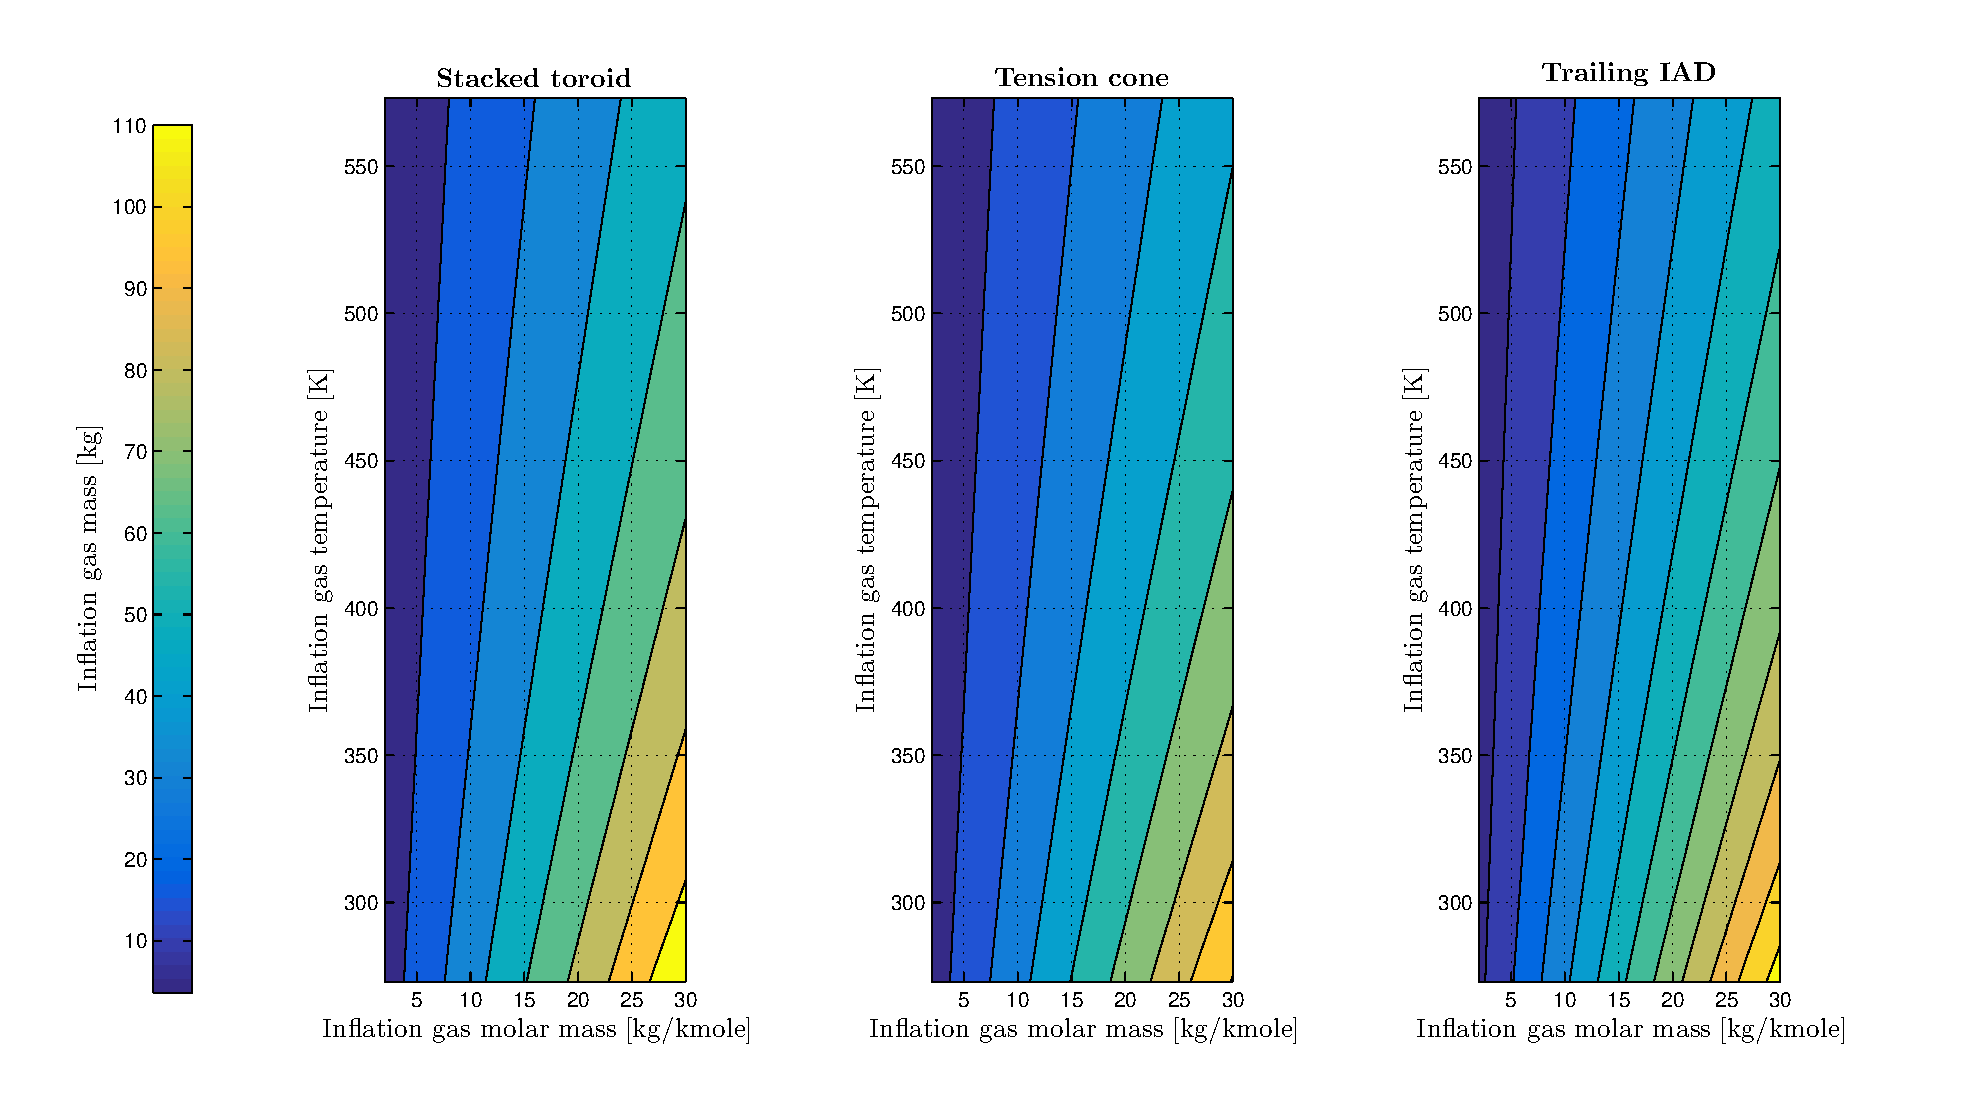
\includegraphics[width = 1.1\textwidth]{Figure/gas_temp_mass.eps}
\caption{Inflation gas mass as a function of gas temperature and molar mass of the stacked toroid, tension cone and trailing ballute configurations}
\label{fig:inflmass}
\end{figure}

Fig.\ref{fig:inflmass} confirms that a denser gas, characterized by a higher molar mass, yields a larger inflation gas mass. An overview of gas generator types and their output is given on page 7 by Brown \cite{Brown2003}. A typical molar mass is that of nitrogen, 22 [$\frac{kg}{mole}$], used in the IRVE satellites \cite{Dillman2012}. It should be noted that inflation system mass is typically estimated as a percentage of inflation gas mass. Total inflation system mass, thus consisting of inflation system and inflation gas mass, will therefore not be as low as suggested by Fig.\ref{fig:inflmass} for low molar mass inflation gases, but it will typically be higher by requiring a heavier inflation system \cite{Brown2003}. Inflation gas mass decreases for an increasing inflation gas temperature, again conforming to expectations. Via the ideal gas law the mass occupied by a certain number of moles of inflation gas will increase for a decreasing temperature through an increased gas density \cite{AndersonJr.2007}.

\subsubsection{Number of toroids for the stacked toroid configuration}
The stacked toroid features a number of toroids that are inflated. To investigate the effect of the number of toroids on total structural decelerator mass, the two are plotted against one another in Fig.\ref{fig:toro}. 

\begin{figure}[H]
\centering
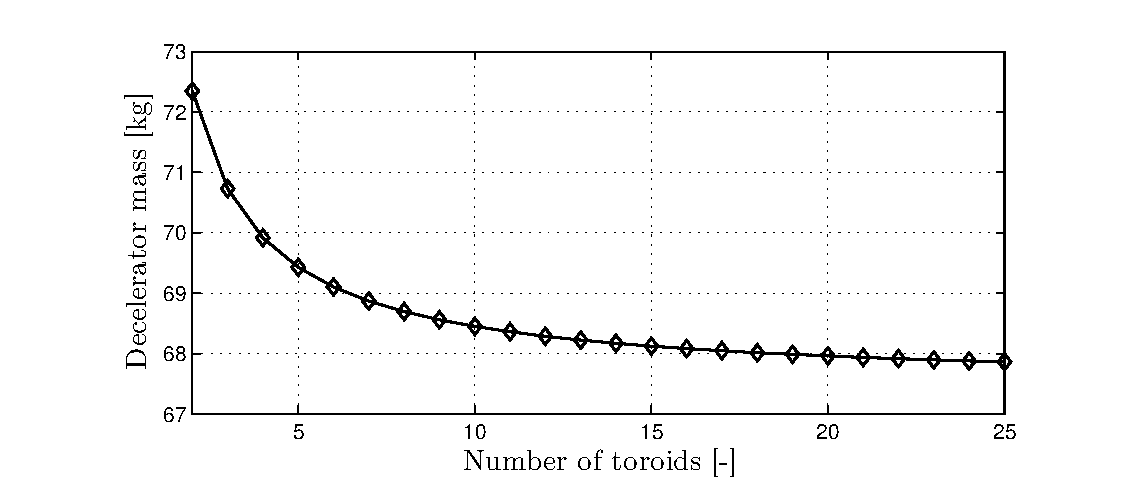
\includegraphics[width = 1.0\textwidth]{Figure/mass_toroids.eps}
\caption{Decelerator structural mass as a function of the number of toroids for the stacked toroid configuration, for a peak dynamic pressure of 3000 [Pa], \gls{sym:CD}= 1.5 [-] and a deployed diameter of 12 [m]}
\label{fig:toro}
\end{figure}

From Fig.\ref{fig:toro}, it may be observed that stacked toroid structural mass decreases for an increasing number of toroids. The decrease is, however, so slight as to be insignificant. A mass decrease of approximately 4 $\%$ is effected by an increase from one to five toroids; a decrease of approximately 5 $\%$ for an increase from one to ten toroids. As the number of toroids is increased beyond ten, mass is more or less constant. Total structural decelerator mass is therefore deemed indifferent to the number of toroids. Care should still be taken to attach too much value to the results yielded by the model, given its limited fidelity.

\subsubsection{Inflatable decelerator diameter}
Figures \ref{fig:mass_dia} and \ref{fig:bc_dia} illustrate the effect of a change in inflatable decelerator diameter on its structural mass. Fig.\ref{fig:mass_dia} illustrates that an increase in deployed diameter, given a certain peak dynamic pressure and drag coefficient, effects an exponential increase in decelerator mass. This increase is significant, adding as much as 33 $\%$ of structural mass for a tension cone for an increase in diameter from 13 to 14 [m], for a peak dynamic pressure of 3000 [Pa] and a drag coefficient of 1.5 [-]; the other concepts exhibit similar increases. A better estimate of the mass-effectiveness for an increasing diameter is given by Fig.\ref{fig:bc_dia}, which displays the ballistic coefficient of the decelerator, taking into account only its structural mass. This figure shows that the ballistic coefficient increases with increasing diameter for stacked toroid, tension cone and trailing ballute, denoting that decelerator structural mass increases more than its decelerating capability (the product of \gls{sym:CD} and \gls{sym:A_iad}) and thus that it becomes less mass-effective for an increasing deployed diameter.

 For the isotensoid configuration a small decrease in ballistic coefficient with increasing deployed diameter may be noted. This follows from the minimum gage thickness requirements incorporated in \gls{sym:df}. As discussed in section \ref{sec:strucmeth} the isotensoid analysis is based on the parameter \gls{sym:df}. This is given as a maximum of the areal density or \gls{sym:df} as computed based on strength requirements of the material using the strength to mass ratio of the material ( \gls{sym:kf}). In the case of the isotensoid design it must be noted that in figure … the mass is based on minimum gage thickness requirements using the areal density of the material. This can be considered as suboptimal performance as rather the materials strength to mass ratio is considered for structural sizing. This suboptimal performance is the reasons that the ballistic coefficient increases rather than decreases for the isotensoid configuration



\begin{figure}[H]
\centering
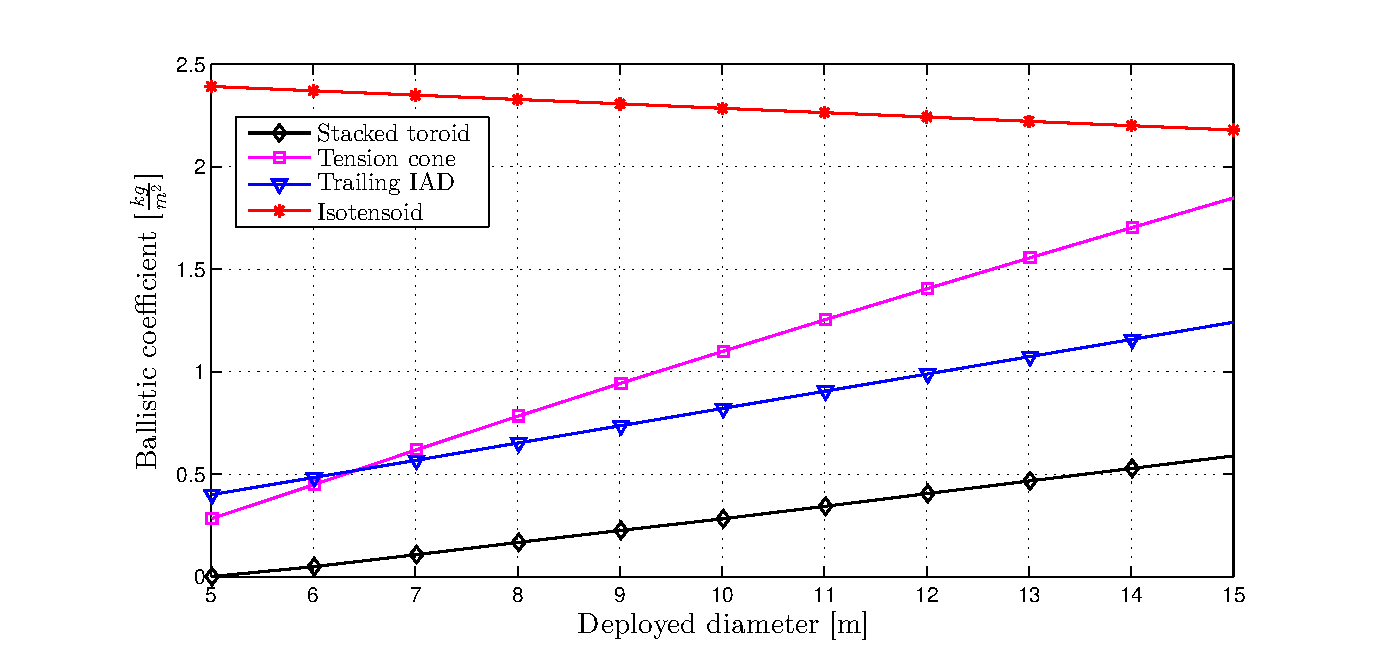
\includegraphics[width = 1.0\textwidth]{Figure/bc_dia.eps}
\caption{Decelerator structural ballistic coefficient as a function of deployed diameter of inflatable concepts for a peak dynamic pressure of 3000 [Pa] and \gls{sym:CD}= 1.5 [-]}
\label{fig:bc_dia}
\end{figure}

\subsubsection{Half-cone angle}
Figures \ref{fig:mass_theta_cd} and \ref{fig:bc_theta_cd} display how the structural ballistic coefficient of the decelerator changes with half-cone angle and drag coefficient. Similar figures result if the peak dynamic pressure is taken as a variable rather than the drag coefficient, which conforms to expectations given that peak dynamic pressure and drag coefficient features almost exclusively as a product. From Fig.\ref{fig:mass_theta_cd}, it can be observed that mass increases for an increasing half-cone angle (and an increasing drag coefficient). From  Fig.\ref{fig:bc_theta_cd}, it can be observed that mass-effectiveness (reflected by the ballistic coefficient of the decelerator structural mass) has an optimum with respect to the half-cone angle. This optimum is well established for stacked toroid and tension cone configurations, but disappears as the drag coefficient is increases for the trailing ballute configuration.

For a drag coefficient of 1.5 [-], the optimum is located at approximately 60 [deg] for the stacked toroid configuration; at approximately 55 [deg] for the tension cone configuration. Except for the trailing ballute configuration, this optimum angle is more or less maintained. A study by Brown et al \cite{Brown2003}, using a parametric mass model based on the sizing of the structure to prevent buckling (different from the model used for the production of Fig.\ref{fig:bc_theta_cd}), finds a mass-optimum cone angle of 55 [deg] for a hypercone (comparable to the tension cone concept) \cite[p.6]{Brown2003}. Brown et al, however, establish this angle as having minimum hypercone mass, rather than maximum mass-efficiency. 
\begin{figure}[H]
\centering
\includegraphics[width = 0.92\textwidth]{Figure/mass_theta_cd.eps}
\caption{Decelerator structural mass as a function of half-cone angle and drag coefficient of inflatable concepts, for a peak dynamic pressure of 3000 [Pa] and a deployed diameter of 12 [m]}
\label{fig:mass_theta_cd}
\end{figure}

\begin{figure}[H]
\centering
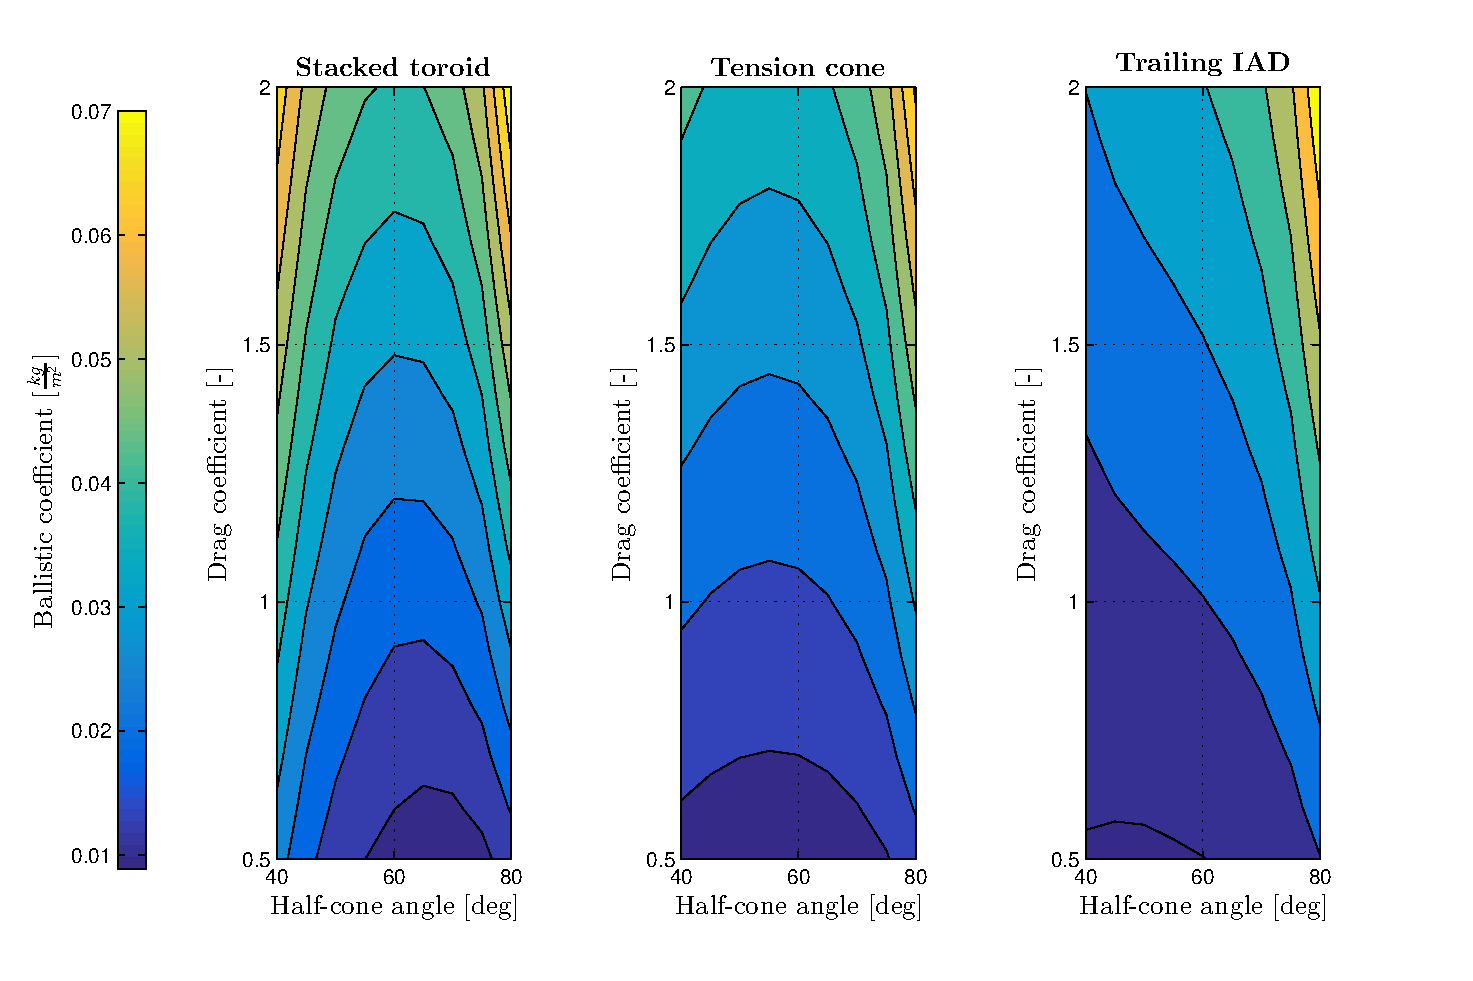
\includegraphics[width = 0.92\textwidth]{Figure/bc_theta_cd.eps}
\caption{Decelerator structural ballistic coefficient as a function of half-cone angle and drag coefficient of inflatable concepts, for a peak dynamic pressure of 3000 [Pa] and a deployed diameter of 12 [m]}
\label{fig:bc_theta_cd}
\end{figure}